\section {Числовые характеристики случайных величин: квантили. Медиана и ее свойства. Интерквартильный размах}

\begin{defn}
    \textit{Медианой} $\operatorname{Med} \xi$ распределения случайной величины $\xi$ называется любое из \textit{чисел} $\mu$ таких, что
    \begin{equation*}
        \myprob{\xi \leqslant \mu} \geqslant \frac{1}{2}, ~~~ \myprob{\xi \geqslant \mu} \geqslant \frac{1}{2}.
    \end{equation*}
\end{defn} 

\begin{rmrk}
    Медиана распределения всегда существует, но может быть не единственна. 
    Например, в случае дискретного распределения $\mathbb{P}(\xi = -1) = \mathbb{P}(\xi = 1) = \frac{1}{2}$ и $1$, и $-1$ удовлетворяют определению медианы.
\end{rmrk} 

\begin{defn}
\textit{Квантиль порядка $\gamma$}~--- это такое число $\kappa_\gamma$, для которого выполняется 
$$ \begin{cases} 
    \myprob{\xi \leqslant \kappa_\gamma} = F(\kappa_\gamma) & \geqslant \gamma, \\
    \myprob{\xi \geqslant \kappa_\gamma} = 1 - F(\kappa_\gamma + 0) & \geqslant 1 - \gamma 
\end{cases}
$$
\end{defn}

\begin{rmrk}
    Если функция распределения $F$ непрерывна и строго монотонна, то \textit{квантилем} порядка (уровня) $\gamma$, где $\gamma \in (0; 1), $ является решение $x_\gamma$ уравнения $F(x_\gamma) = \gamma.$ 
    Тогда квантиль порядка $\gamma$ отрезает от области под графиком плотности область с площадью $\gamma$ слева от себя. Справа от $\kappa_\gamma$ площадь области равна $1 - \gamma$.
    
    Если же случайная величина не является абсолютно непрерывной, то уравнение $F(x_\gamma) = \gamma$ может не иметь решений. Например, для приведенного ниже графика не существует $x_{\frac{1}{2}}: F(x_{\frac{1}{2}}) = \frac{1}{2}$.
        
    \medskip\hfill\break
    \begin{center}
    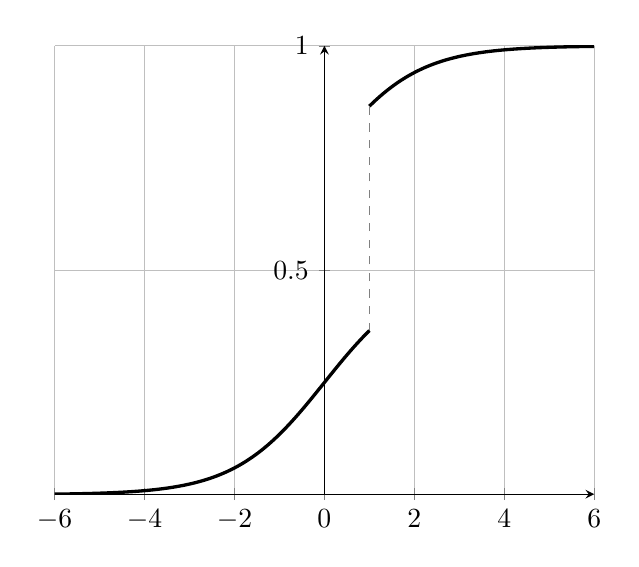
\begin{tikzpicture}[declare function={sigma(\x)=1/(1+exp(-\x));}]
    \begin{axis}
    [
        grid=major,     
        xmin=-6,
        xmax=6,
        axis x line=bottom,
        ytick={0,.5,1},
        ymax=1,
        axis y line=middle,
        samples=100,
        domain=-6:6,
        legend style={at={(1,0.9)}}     
    ]
        \draw [dashed,black!50] (1,0.365) -- (1,0.865);
        \addplot[very thick,black,mark=none, samples=100,domain=-6:1]   (x, {.5 * sigma(x)});
        \addplot[very thick,black,mark=none, samples=100,domain=1:6]   (x, {.5 + .5 * sigma(x)});
    \end{axis}
    \end{tikzpicture}
    \end{center}
\end{rmrk} 

\begin{defn}
    Квантили уровней, кратных $0.01$, называют \textit{процентилями}, квантили уровней, кратных $0.1$, — \textit{децилями}, уровней, кратных $0.25$, — \textit{квартилями}.
\end{defn} 

\begin{rmrk}
    Медиана является квантилем уровня $1 / 2$.
\end{rmrk} 

\begin{namedthm}[Свойства медианы]\leavevmode
\begin{enumerate}
    \item Медиана случайной величины $\xi$ минимизирует средний модуль её отклонения:
    \begin{equation*}
        \mathbb{E}|\xi - \operatorname{Med} \xi| 
    = \min _{a} \mathbb{E}|\xi-a|;
    \end{equation*}
    \item Отклонение медианы случайной величины $\xi$ от её математического ожидания $\mathbb{E}\xi$ не превышает по модулю среднеквадратичного отклонения $\sigma = \sqrt{\mathbb{D}\xi}$:
    \begin{equation*}
        |\mathbb{E}\xi - \operatorname{Med}\xi| \leqslant \sigma.
    \end{equation*}
\end{enumerate}
\end{namedthm}

\begin{proof}
    \begin{enumerate}
        \item Рассмотрим случайную величину $\eta = \xi - \operatorname{Med}\xi$. 
        Очевидно, что $\operatorname{Med} \eta = 0$. 
        Тогда нам надо показать, что $\forall \, c \in \mathbb{R} $ справедливо 
        \begin{equation*}
            \mathbb{E} |\eta - c| - \mathbb{E}|\eta| \geqslant 0.
        \end{equation*}
        
        Рассмотрим случай $c > 0$. Заметим, что 
        \begin{gather*}
            |\eta - c| - |\eta| = c, \quad \eta < 0 \\
            |\eta - c| - |\eta|  \geqslant -c, \quad \eta \geqslant 0.
        \end{gather*}
        Тогда
        \begin{gather*}
            \mathbb{E} \bigl(|\eta - c| - |\eta| \bigl) 
            = \mathbb{E} \bigl( (|\eta - c| - |\eta|) \cdot \mathrm{I}(\eta < 0) + (|\eta - c| - |\eta|) \cdot \mathrm{I}(\eta \geqslant 0) \bigl) \\
            \mathbb{E} \bigl( |\eta - c| - |\eta| \bigl) \geqslant c~\mathbb{P}(\eta < 0) - c~\mathbb{P}(\eta \geqslant 0).
        \end{gather*}
        Так как $\operatorname{Med}\eta = 0$, то $\mathbb{P}(\eta \leqslant 0) = \mathbb{P}(\eta \geqslant 0) = \frac{1}{2}$.
        Отсюда вытекает
        \begin{equation*}
            \mathbb{E}\bigl( |\eta - c| - |\eta| \bigl) \geqslant 0.
        \end{equation*}
        Случай $c < 0$ сводится к предыдущему умножением случайной величины и $c$ на $-1$. Отсюда следует, что медиана действительно минимизирует средний модуль отклонения.
        \item Рассмотрим цепочку неравенств:
        \begin{align*}
            |\mathbb{E}\xi - \operatorname{Med}\xi| =
            |\mathbb{E}\left[ \operatorname{Med}\xi - \xi \right]| & \leqslant 
            {\text{\{шестое св-во мат. ожидания\}}} \\ \leqslant 
            \mathbb{E} |\operatorname{Med}\xi - \xi| & \leqslant 
            {\text{\{первое св-во медианы\}}} \\ \leqslant
            \mathbb{E}| \mathbb{E}\xi - \xi| = 
            \mathbb{E} \sqrt{|\mathbb{E}\xi - \xi|^2} & \leqslant
            {\text{\{неравенство Йенсена\}}} \\ \leqslant 
            \sqrt{\mathbb{E}| \mathbb{E}\xi - \xi|^2} & = 
            \sqrt{\mathbb{D}\xi} = \sigma.
        \end{align*}
    \end{enumerate}
\end{proof}

\subsubsection{Интерквантильный размах}

\begin{defn}
    \textit{Интерквартильным размахом} называется разность между третьим и первым квартилями, то есть ${\displaystyle x_{0{,}75}-x_{0{,}25}}.$
\end{defn} 

В каком-то смысле эту величину можно считать аналогом дисперсии случайной величины, устойчивой к выбросам.
